% !TEX program = xelatex
\documentclass[cn,11pt,a4paper,founder]{elegantpaper}

\usepackage{mathtools}
\let\Bbbk\undefined
\usepackage[complete,subscriptcorrection,slantedGreek]{mtpro2} 
\usepackage[most]{tcolorbox}

\newcommand{\mt}[1]{\CJKfontspec{MaoTi-Regular}#1}
\newcommand{\calJ}{\mathcal{J}}
\newcommand{\calR}{\mathcal{R}}
\newcommand{\calH}{\mathcal{H}}
\newcommand{\calN}{\mathcal{N}}
\newcommand{\calD}{\mathcal{D}}
\newcommand{\calE}{\mathcal{E}}
\newcommand{\bbC}{\mathbb{C}}
\newcommand{\bbR}{\mathbb{R}}
\newcommand{\ept}{\hspace{2.85pt}}
\newcommand{\upcite}[1]{\textsuperscript{\textsuperscript{\cite{#1}}}} 
\renewcommand{\b}{\boldsymbol}
\renewcommand{\thetable}{\thesection{}.\arabic{table}}
\renewcommand{\thefigure}{\thesection{}.\arabic{figure}}
\renewcommand{\theequation}{\thesection{}.\arabic{equation}}
\colorlet{LightLavender}{red!30!}
\renewcommand{\emph}[1]{{\fontspec{TimesNewRomanPS-BoldMT}\heiti{#1}}}
\tcbset{
		on line,
		left=0pt, right=0pt, top=0pt, bottom=0pt,
		colframe=white, colback=LightLavender, 
		highlight math style={enhanced}
}
\DeclareMathOperator{\tr}{tr}
\DeclareMathOperator{\RP}{Re}
\DeclareMathOperator{\spans}{span}
\DeclareMathOperator{\transpose}{T}

\hypersetup{
		pdftitle = {Optimal dual frames for erasures},
		pdfauthor = {李徐瑾},
		pdfkeywords = {最佳对偶框架},
		pdfsubject = {数值代数论文翻译}
}


\title{丢失问题下的最佳对偶框架\\
Optimal dual frames for erasures}
\author{\kaishu{作者}: Jerry Lopez and Deguang Han\\
\mt{中佛罗里达大学数学系}\\
\kaishu{翻译}: 李徐瑾\\
\mt{电子科技大学数学科学学院}}
\date{\zhtoday}


\begin{document}

\maketitle

\begin{abstract}
对有限维Hilbert空间中任给的框架,我们研究该框架的最佳对偶框架的丢失问题. 证明了典范对偶不一定是最佳的. 且最佳对偶框架不一定是唯一的. 给出了典范对偶是丢失问题的唯一最佳对偶框架的几个充分条件. 作为应用,当框架是由群表示诱导或一致紧时,典范对偶框架是唯一的最佳对偶框架.
\keywords{框架,丢失,最佳对偶框架}
\end{abstract}

\section{介绍}
近年来,从编码理论的角度寻找“最佳紧框架”一直是广大研究者的兴趣所在. 这导致了人们对最佳框架丢失问题的研究\upcite{en02,en03,en04,en06,en10,en15,en16,en17}. 通常在处理信号丢失时,在信号编码之前会找到最佳框架,这可以最大限度地减小重构具有一定数量丢失坐标时的编码信号的错误. 然后使用最佳框架对信号(向量)进行编码和解码. 已知均匀长度的紧框架在\(1\)丢失的条件下是最佳的,并且等角框架在\(2\)丢失的情况下是最佳的\upcite{en15}. 本论文我们另辟蹊径: 我们的场景是使用一个已选定的(不一定是紧的)框架来进行编码,然后,若存在丢失的坐标,则使重构误差最小化来重构的对偶框架中的向量. 这种对偶框架被称为关于丢失的\emph{最佳对偶框架}. 为了讨论我们的主要结论,我们首先回顾并介绍一些Hilbert空间中框架的符号和定义.

可分(实或复)的Hilbert空间\(\calH\)中的\emph{框架}意即\(\calH\)中的序列\(\{x_j\}_{j\in\calJ}\)对于任一\(x\in\calH\)使得
\[
	A\|x\|^2\leqslant\sum_{j\in\calJ}|\langle x,x_j\rangle|^2\leqslant B\|x\|^2,\quad\forall A,B>0.
\]
最佳常数(\(A\)的极大值和\(B\)极小值)称为\emph{框架界}. 若\(A=B\),则称框架为\emph{紧框架}. 若\(A=B=1\),则称框架为\emph{Parseval框架}. (有时Parseval框架也称为\emph{规范紧框架}). 若框架序列的全体元素均有相同的范数,则称框架为\emph{均匀框架}. 若框架\(\{x_j\}_{i\in\calJ}\)满足\(|\langle x_i,x_j\rangle|=c_i,\forall i\ne j\),则称框架为\emph{等角框架}. Parseval等角框架的存在对\(\calJ\)的基数和Hilbert空间的维数有严格的限制\upcite{en17}.

对于\(\calH\)的一个框架\(\{x_j\}_{j\in\calJ}\),定义\emph{分析算子}为线性映射\(\Theta\colon\calH\to\ell^2(\calJ)\),即
\[
	\Theta(x)=\sum_{j\in\calJ}\langle x,x_j\rangle e_j,
\]
其中\(\{e_j\}_{j\in\calJ}\)是\(\ell^2(\calJ)\)中的标准正交基. \(\Theta\)的伴随算子\(\Theta^{\star}\)为
\[
	\Theta^{\star}\bigg(\sum_{j\in\calJ}c_j e_j\bigg)=\sum_{j\in\calJ}c_i x_i.
\]
若设\(S=\Theta^{\star}\Theta\),则有
\[
	Sx=\sum_{j\in\calJ}\langle x,x_j\rangle x_j,\quad x\in\calH.
\]
因此\(S\)是\(\calH\)上的一个正可逆有界线性算子,称为\(\{x_j\}_{j\in\calJ}\)的\emph{框架算子}. 直接计算得出
\begin{align*}
x&=\sum_{j\in\calJ}\langle x,S^{-1/2}x_i\rangle S^{-1/2}x_j\\
&=\sum_{j\in\calJ}\langle x,S^{-1}x_j\rangle x_j\\
&=\sum_{j\in\calJ}\langle x,x_j\rangle S^{-1}x_j,\quad x\in\calH.
\end{align*}
这表明\(\{S^{-1/2}x_j\}_{j\in\calJ}\)是\(\calH\)的一个Parseval框架且\(\{S^{-1}x_j\}_{j\in\calJ}\)也是\(\calH\)的一个框架. 框架\(\{S^{-1}x_j\}_{j\in\calJ}\)称为\(\{x_j\}_{j\in\calJ}\)的\emph{典范(标准)对偶框架},用于用编码系数序列\(\{\langle x,x_j\rangle\}_{j\in\calJ}\)重构信号\(x\).

在本文中,我们只对具有有限多个向量的框架感兴趣,因此Hilbert空间默认是有限维的.

当\(\calH=\bbC^k\)或\(\bbR^k\),框架\(\{x_j\}_{j=1}^k\)的分析算子是\(n\times k\)阶矩阵,其中第\(j\)行的行向量为\(x_j=(x_{j1},x_{j2},\cdots,x_{jk})\). 
设\(\eta_i,i=1,2,\cdots,k\)表示分析矩阵的列向量. 则\(\calR(\Theta)=\spans\{\eta_i\}_{i=1}^k\). 于是我们有
\begin{enumerate}[(i)]
\item \(\{x_i\}_{i=1}^n\)是一个框架当且仅当\(\Theta\)的列向量线性无关.
\item \(\{x_i\}_{i=1}^n\)是一个规范紧框架当且仅当\(\Theta\)的列向量构成一组正交集.
\item \(\{x_i\}_{i=1}^n\)是一个均匀长度框架当且仅当\(\Theta\)的列向量线性无关且行向量具有相同的\(\ell^2\)范数.
\end{enumerate}

给定\(k\)维Hilbert空间中的一个有限框架\(\{x_i\}_{i=1}^n\). 则必有\(n\geqslant k\). 当\(n>k\)时,除了典范对偶框架之外,仍然存在无穷多个\(\calH\)中的框架\(\{y_i\}_{i=1}^n\)构成了\(\calH\)中的重构法则:
\[
	x=\sum_{i=1}^n\langle x,x_i\rangle y_i,\quad x\in\calH.
\]
满足上述重构法则的框架\(\{y_i\}_{i=1}^n\)称为\emph{替代对偶框架}或者简称为\(\{x_i\}_{i=1}^n\)的\emph{对偶框架}. 典范对偶与替代对偶之间的联系可表述为: \(\{y_i\}_{i=1}^n\)时\(\{x_i\}_{i=1}^n\)的替代对偶当且仅当
\[
	y_i=S^{-1}x_i+h_i,\quad\forall 1\leqslant i\leqslant n,
\]
其中\(\{h_i\}_{i=1}^n\)满足条件
\[
	\sum_{i=1}^n\langle x,x_i\rangle h_i=0,\quad\forall x\in\calH.
\]
为了便于表述,我们使用\tcbox{\((n,k)\)-\text{框架}}来表示\(k\)维Hilbert空间\(\calH\)中具有\(n\)个元素的一个框架,使用\tcbox{\((n,k)\)-\text{对偶框架对}}来表示\(k\)维Hilbert空间\(\calH\)中具有\(n\)个元素的一个对偶框架对.

在编码理论中,一个向量(信号)\(x\)在框架\(\{x_i\}_{i=1}^n\)中被编码为\(\Theta(x)=\{\langle x,x_i\rangle\}_{i=1}^n\),接着\(\Theta(x)\)发送给一个接收器来解码恢复信号\(x\). 最后的解码过程需由对偶框架完成. 然而,在传输过程中编码数据\(\Theta(x)\)的一些系数或许会丢失. 鉴于框架的冗余性(当\(n>k\)时),任有可能在原来信号\(x\)丢失少量数据的基础上完美恢复信号. 但实际上在接收端进行重构是不可行的,这会导致重构严重依赖于数据丢失的位置. 由于该问题的存在,我们使用框架\(\{x_i\}_{i=1}^n\)的典范对偶框架来近似\(x\),即
\[
	\bar{x}=\sum_{i\in\Lambda_x}\langle x,x_i\rangle S^{-1}x_i,
\]
其中\(\Lambda_x\)表示全体\(\langle x,x_i\rangle\)接收到的信号. 目的是选取一个框架使得误差\(x-\bar{x}\)极小(在某种度量的意义下). 为了准确起见,我们首先介绍\emph{误差算子},是对Parseval框架采用的一种表示法\upcite{en15}. 设\(\calD_m\)是全体\(n\times n\)阶对角矩阵所组成的集合,其中\(m\)个对角元为\(1\),\(n-m\)个对角元为\(0\). 对于任意的对偶框架对\((X,Y)\)且\(X=\{x_i\}_{i=1}^n,Y=\{y_i\}_{i=1}^n\),我们定义
\begin{equation}\label{eq:1.1}
d_m(X,Y)\coloneqq\max\{\|\Theta_Y^{\star}D\Theta_X\|\mid D\in\calD_m\},
\end{equation} 
其中\(\Theta_X\)和\(\Theta_Y\)分别是\(X\)和\(Y\)的分析算子且\(\|\cdot\|\)表示矩阵(算子)范数. 若\(J=\{i_1,i_2,\cdots,i_m\}\)表示对角矩阵\(D\)中对角元为\(1\)所对应的指标. 则当由\(\bar{x}=\sum_{j\notin J}\langle x,x_j\rangle y_j\)逼近\(x\)时,对于给定的\(m\)丢失的误差算子\(E_j\)为
\begin{align*}
E_j x&=(\Theta_Y^{\star}D\Theta_X)(x)\\
&=x-\sum_{j\notin J}\langle x,x_i\rangle y_i\\
&=\sum_{i=1}^n\langle x,x_i\rangle y_i-\sum_{j\notin J}\langle x,x_j\rangle y_j\\
&=\sum_{j\in J}\langle x,x_j\rangle y_j.
\end{align*}
因此误差算子\(\Theta_Y^{\star}D\Theta_X\)的测度衡量了逼近的近似程度. 当使用算子范数时,一个最佳对偶框架对可定义为: 一个\((n,k)\)-对偶框架对\((\tilde{X},\tilde{Y})\)被称为\tcbox{对\(m\)丢失最佳},若其对\((m-1)\)丢失最佳且\(d_m(\tilde{X},\tilde{Y})\)使得\(d_m(X,Y)\)对于全体\((n,k)\)-对偶框架对极小. 当全体\((n,k)\)-Parseval框架满足\(Y=X\)时,许多研究人员证明,Parserval框架\(\{x_i\}_{i=1}^n\)对\(1\)丢失最佳当且仅当此框架是均匀的,对\(2\)丢失最佳当且仅当此框架是等角均匀框架(在\((n,k)\)-框架存在的条件下). 当使用\(\Theta_Y^{\star}D\Theta_X\)的光谱半径度量时,对于一般的最佳对偶框架对也有非常相似的结果\upcite{en15}.

在实际应用中,在选择框架进行编码时可能有很多限制. 例如,鉴于实际应用中的需要,某些极不规范的框架可能更适合编码(与等角框架、均匀框架和Parseval框架等对比而言). 这导致了为给定框架选择“最佳”对偶框架的问题,使得该对偶框架在发生丢失时误差极小. 由于我们研究的是有限维空间,最佳对偶框架总是存在的(参见推论\ref{co:2.2}). 然而,与存在噪声的一些重构问题\upcite{en01}中典范对偶是最佳选择相反,典范对偶一般不一定是丢失问题的最佳选择(参加第\ref{sec:3}节的范例). 这就引出了一个问题,即如何识别某些类型的框架,使得典范对偶框架是丢失问题的最佳框架. 在第\ref{sec:2}节我们证明了在\(\|x_i\|\cdot\|S^{-1}x_i\|=c_i,\forall 1\leqslant i\leqslant n\)的条件下(其中\(S\)是框架算子),框架\(\{x_i\}_{i=1}^n\)的典范框架是该框架丢失问题的最佳框架. 做为应用,我们得到典范对偶框架对由群表示诱导的每一个框架都是最佳的. 这对于均匀紧框架也是成立的.

\section{最佳对偶框架}\label{sec:2}
设\(X=\{x_i\}_{i=1}^n\)是\(\calH\)的\((n,k)\)维框架且\(d_m(X,Y)\)如式\eqref{eq:1.1}所定义. 我们称\(Y=\{y_i\}_{i=1}^n\)是\(X\)在\(1\)丢失条件下的一个最佳对偶框架,若
\[
	d_1(X,Y)=\min\{d_1(X,Z)\mid Z\ept\text{是}\ept X\ept\text{的对偶框架}\}.
\]
更一般地,\(X\)的对偶框架\(Y\)称为在\(m\)丢失下的一个最佳对偶框架,若其对\((m-1)\)丢失是最佳的且
\[
	d_m(X,Y)=\min\{d_m(X,Z)\mid Z\ept\text{是}\ept X\ept\text{的对偶框架}\}.
\]

我们注意到\(m\)丢失的最佳对偶亦是\((m-1)\)的最佳丢失,丢失问题通常需寻求一个替代对偶使得\(m\)个数据丢失的损失最小.

设\(S\)是\(X\)的框架算子. 则\(Y=\{y_i\}_{i=1}^n\)是\(X\)的对偶框架当且仅当\(Y=S^{-1}X+U\)且
\[
	\sum_{i=1}^n\langle x,x_i\rangle u_i=0,\quad\forall x\in\calH,
\]
其中\(U=\{u_1,u_2,\cdots,u_n\}\),满足\(\Theta_U^{\star}\Theta_X=0\),且\(\Theta_U\)和\(\Theta_X\)分别是\(U\)和\(X\)的分析算子. 定义
\[
	\calN_X\coloneqq\{U=\{u_i\}_{i=1}^n\mid\Theta_U^{\star}\Theta_X=0\}.
\]
由于\(\Theta_{S^{-1X}}=\Theta_{X}S^{-1}\),我们立得\(X\)在\(m\)丢失条件下的一个最佳对偶框架将是下列极小极大问题的一个解:
\[
	\min_{U\in\calN_X}\max\big\{\|S^{-1}\Theta_X^{\star}D\Theta_X+\Theta_U^{\star}D\Theta_X\|\mid D\in\calD_m\big\}.
\]

我们首先证明任意丢失的对偶框架的存在性. 设\(x,y\in\calH\). 我们用\(x\otimes y\)表示秩一算子,定义为\((x\otimes y)(v)=\langle v,y\rangle x,\forall v\in\calH\).

注意到,若\(D\in\calD_1\)且\(Y=\{S^{-1}x_i+u_i\}_{i=1}^n\),其中\(U=\{u_i\}_{i=1}^n\in\calN_X\), 则有
\[
	\|\Theta_Y^{\star}D\Theta_X\|=\big\|(S^{-1}x_i+u_i)\otimes x_i\big\|=\big\|(S^{-1}x_i+u_i)\big\|\cdot\|x_i\|,
\]
其中\(1\leqslant i\leqslant n\). 因此当我们考虑\(1\)丢失的最佳对偶框架时,不妨假设\(x_i\ne 0,\forall 1\leqslant i\leqslant n\). 故函数\(F(U)\)定义为
\[
	F(U)\coloneqq d_1(X,S^{-1}X+U)=\max\big\{\|(S^{-1}x_i+u_i)\|\cdot\|x_i\|\mid\forall 1\leqslant i\leqslant n\big\}
\]
是关于\(U\)的连续函数满足\(\lim_{\|U\|\to\infty}F(U)=0\),其中\(U\)由Hilbert空间\(\calH^{(n)}\coloneqq\calH\oplus\calH\oplus\cdots\oplus\calH\)中的正交向量构成.

\begin{lemma}\label{le:2.1}
设\(X=\{x_i\}_{i=1}^n\)是\(\calH\)的一个框架且\(x_i\ne 0,\forall 1\leqslant i\leqslant n\). 则存在\(X\)在\(1\)丢失条件下的最佳对偶框架. 更进一步地,全体\(X\)在\(m\)丢失条件下的最佳对偶框架组成的集合是\(\calH^{(n)}\)的闭凸有界子集.
\end{lemma}

\begin{proof}
我们仅需证明集合的凸性. 设\(Y^{(1)}\)和\(Y^{(2)}\)是\(X\)在\(m\)丢失条件下的两个最佳对偶框架. 则有
\[
	d_m\big(X,Y^{(1)}\big)=d_m\big(X,Y^{(2)}\big)=\min\{d_m(X,Z)\mid Z\ept\text{是}\ept X\ept\text{的对偶框架}\}.
\]
设\(Y=\lambda Y^{(1)}+(1-\lambda)Y^{(2)},\forall\lambda\in[0,1]\). 显然\(Y\)是\(X\)的对偶. 仅需证明
\[
	d_m(X,Y)=d_m\big(X,Y^{(1)}\big)=d_m\big(X,Y^{(2)}\big).
\] 
事实上,对于任意的\(D\in\calD_m\),我们有
\begin{align*}
\|\Theta_Y^{\star}D\Theta_X\|&=\big\|\lambda\Theta_{Y^{(1)}}^{\star}D\Theta_X+(1-\lambda)\Theta_{Y^{(2)}}^{\star}D\Theta_X\big\|\\
&\leqslant\lambda\big\|\Theta_{Y^{(1)}}^{\star}D\Theta_X\big\|+(1-\lambda)\big\|\Theta_{Y^{(2)}}^{\star}D\Theta_X\big\|\\
&\leqslant\lambda d_m\big(X,Y^{(1)}\big)+(1-\lambda)d_m\big(X,Y^{(2)}\big)\\
&=d_m\big(X,Y^{(1)}\big)\\
&=d_m\big(X,Y^{(2)}\big).
\end{align*}
因此
\[
	d_m(X,Y)\leqslant d_m(X,Y^{(1)})=d_m(X,Y^{(2)}).
\]
故等式成立.
\end{proof}

\begin{corollary}\label{co:2.2}
设\(X=\{x_i\}_{i=1}^n\)是\(\calH\)的一个框架且\(x_i\ne 0,\forall 1\leqslant i\leqslant n\). 则存在\(X\)在\(m\)丢失条件下的最佳对偶框架. 更进一步地,全体\(X\)在\(m\)丢失条件下的最佳对偶框架组成的集合是\(\calH^{(n)}\)的闭凸有界子集.
\end{corollary}

\emph{Mercedes-Benz框架}是最佳典范框架的一个简单范例:

\begin{example}\label{ex:2.3}
设\(\calH=\bbR^2\),考虑框架\(X=\{x_i\}_{i=1}^3\),即
\[
	\left\{\begin{bmatrix}
	1\\
	0
	\end{bmatrix},
	\begin{bmatrix}
	-1/2\\
	\sqrt{3}/2
	\end{bmatrix},
	\begin{bmatrix}
	-1/2\\
	-\sqrt{3}/2
	\end{bmatrix}\right\}.
\]
事实上,此框架是由一个群表示诱导出来的,且典范对偶是唯一的最佳对偶,详见推论\ref{co:2.9}.
\end{example}

接下来,我们给出的两个范例表明一个框架可能有无穷多个最佳对偶框架,且典范对偶无需是最佳的即使最佳对偶是唯一的. 这两个范例的细节将会在第\ref{sec:3}节加以说明.

\begin{example}\label{ex:2.4}
设\(\calH=\bbR^2\),考虑框架\(X=\{x_i\}_{i=1}^3\),即
\[
	\left\{\begin{bmatrix}
	1\\
	0
	\end{bmatrix},
	\begin{bmatrix}
	0\\
	1
	\end{bmatrix},
	\begin{bmatrix}
	1/\sqrt{2}\\
	1/\sqrt{2}
	\end{bmatrix}\right\}.
\]
这是一个均匀的非Parseval的框架,其中\(\|x_i\|=1,\forall 1\leqslant i\leqslant n\). 此框架\(X\)在\(m\)丢失的条件下具有唯一的对偶框架但不是\(X\)的典范对偶的.
\end{example}

\begin{example}\label{ex:2.5}
设\(\calH=\bbR^2\),考虑框架\(X=\{x_i\}_{i=1}^3\),即
\[
	\left\{\begin{bmatrix}
	1\\
	0
	\end{bmatrix},
	\frac{1}{2}\begin{bmatrix}
	0\\
	1
	\end{bmatrix},
	\frac{1}{2}\begin{bmatrix}
	0\\
	1
	\end{bmatrix}\right\}.
\]
则框架\(X\)对于\(1\)丢失和\(2\)丢失具有无穷多个最佳对偶框架.
\end{example}

接下来的结论给我们提供了一大类在任意\(m\)丢失条件下典范对偶框架是唯一的最佳对偶框架.

\begin{theorem}\label{th:2.6}
设\(\{x_i\}_{i=1}^n\)是\(k\)维Hilbert空间\(\calH\)的一个框架且\(S\)是其框架算子. 若满足
\[
	\|S^{-1}x_i\|\cdot\|x_i\|=c_i,\quad\forall 1\leqslant i\leqslant n,
\]
则在任意\(m\)丢失的条件下典范对偶框架是唯一的最佳对偶框架.
\end{theorem}

为了证明定理\ref{th:2.6}需引入如下引理.

\begin{lemma}\label{le:2.7}
设\(\calH\)中的序列\(X=\{x_i\}_{i=1}^n\)和\(U=\{u_i\}_{i=1}^n\)使得\(\Theta_U^{\star}\Theta_X=0\). 则\(\sum_{i=1}^n\langle x_i,u_i\rangle=0\).
\end{lemma}

\begin{proof}
事实上,我们有
\begin{align*}
\tr(\Theta_X\Theta_U^{\star})&=\tr(\Theta_U^{\star}\Theta_X)\\
&=\sum_{i=1}^n\langle x_i,u_i\rangle\\
&=0.
\end{align*}
\end{proof}

接下来我们给出定理\ref{th:2.6}的证明.

\begin{proof}
根据\(m\)丢失条件下最佳对偶的定义,易得\(\{S^{-1}x_i\}_{i=1}^n\)是\(1\)丢失条件下唯一的最佳对偶. 设\(\{y_i\}_{i=1}^n=\{S^{-1}x_i+u_i\}_{i=1}^n\)是\(X\)的一个最佳对偶框架,其中\(\Theta_U^{\star}\Theta_X=0\)且\(U=\{u_i\}_{i=1}^n\). 则
\[
	\max_{1\leqslant i\leqslant n}\|S^{-1}x_i+u_i\|\cdot\|x_i\|\leqslant\max_{1\leqslant i\leqslant n}\|S^{-1}x_i\|\cdot\|x_i\|=c=\|S^{-1}x_i\|\cdot\|x_i\|.
\]
因此
\[
	\|y_i\|\cdot\|x_i\|\leqslant\|S^{-1}x_i\|\cdot\|x_i\|,\quad\forall 1\leqslant i\leqslant n.
\]
由于\(x_i\ne 0\),则\(\|y_i\|\leqslant\|S^{-1}x_i\|,\forall 1\leqslant i\leqslant n\). 注意到
\begin{align*}
\|y_i\|^2&=\|S^{-1}x_i+u_i\|^2\\
&=\|S^{-1}x_i\|^2+\|u_i\|^2+2\RP\langle S^{-1}x_i,u_i\rangle,
\end{align*}
则有
\[
	\|u_i\|^2+2\RP\langle S^{-1}x_i,u_i\rangle\leqslant 0,\quad\forall 1\leqslant i\leqslant n.
\]
因此我们有
\[
	\sum_{i=1}^n\|u_i\|^2+2\RP\sum_{i=1}^n\langle S^{-1}x_i,u_i\rangle=\sum_{i=1}^n\Big(\|u_i\|^2+2\RP\langle S^{-1}x_i,u_i\rangle\Big)\leqslant 0.
\]

由于\(\Theta_U^{\star}\Theta_X=0\),则\(\Theta_U^{\star}\Theta_{S^{-1}X}=\Theta_U^{\star}\Theta_X S^{-1}=0\). 根据引理\ref{le:2.7},我们有
\[
	\sum_{i=1}^n\langle S^{-1}x_i,u_i\rangle=0,
\]
因此\(\sum_{i=1}^n\|u_i\|\leqslant 0\),即
\[
	u_i=0,\quad\forall 1\leqslant i\leqslant n.
\]
故\(y_i=S^{-1}x_i\). 这表明在任意\(1\)丢失条件下的典范对偶框架是\(X\)的唯一最佳对偶框架.
\end{proof}

作为特例,我们有以下结论:

\begin{corollary}\label{co:2.8}
若\(X=\{x_i\}_{i=1}^n\)是\(\calH\)的一个紧一致框架,则在任意\(m\)丢失的条件下典范对偶框架是\(X\)的唯一最佳对偶框架.
\end{corollary}

\begin{proof}
假设\(\{x_i\}_{i=1}^n\)是紧框架且框架界为\(A\). 则\(\{x_i\}_{i=1}^n\)的框架算子为\(S=AI\). 因此
\[
	\|S^{-1}x_i\|\cdot\|x_i\|=\frac{1}{A}\|x_i\|^2.
\]
故当\(\{x_i\}_{i=1}^n\)是一致的时,有\(\|S^{-1}x_i\|\cdot\|x_i\|=c_i,\forall 1\leqslant i\leqslant n\). 结论来源于定理\ref{th:2.6}.
\end{proof}

定理\ref{th:2.6}亦可应用于另一类特殊的框架,即由群表示引入的框架. 设\(G\)是一个群. 已知群\(G\)的单正表示\(\pi\)是从群\(G\)到非零Hilbert空间\(\calH_{\pi}\)上的单位算子的同态映射. \(\calH_{\pi}\)称为\emph{表示空间}且\(\dim\calH_{\pi}\)表示空间的维数. 群\(G\)中的一个单正表示\(\pi\)称为一个\emph{框架表示},若存在一个向量\(\varphi\in\calH\)使得\(\{\pi(g)\varphi\mid g\in G\}\)是\(\calH\)的一个框架,此时\(\{\pi(g)\varphi\mid g\in G\}\)称为\emph{G框架}\upcite{en11}. 从框架的定义来看,我们将G框架看成是以G中的元素为指标的序列. G框架显然是均匀框架. 当群\(G\)是一个循环群时,G框架被称为\emph{一般调和框架}\upcite{en06},且当群\(G\)是一个交换群时,G框架被称为\emph{几何均匀框架}\upcite{en07}.

\begin{corollary}\label{co:2.9}
设\(\pi\)是有维群\(G\)在Hilbert空间\(\calH\)上的一个群表示. 若\(\{\pi(g)\varphi\}_{g\in G}\)是\(\calH\)的一个框架,则\(\{\pi(g)\varphi\}_{g\in G}\)的典范框架对于任意的丢失条件均是唯一的最佳对偶框架.
\end{corollary}

\begin{proof}
设\(S\)是\(\{\pi(g)\varphi\}_{g\in G}\)的一个框架算子. 直接计算表明
\[
	S\pi(g)=\pi(g)S,\quad\forall g\in G.
\]
因此
\[
	S^{-1}\pi(g)=\pi(g)S^{-1},\quad\forall g\in G.
\]
即\(S^{-1}\pi(g)\varphi=\pi(g)S^{-1}\varphi\). 故
\[
	\|S^{-1}\pi(g)\varphi\|\cdot\|\pi(g)\varphi\|=\|\pi(g)S^{-1}\varphi\|\cdot\|\pi(g)\varphi\|=\|S^{-1}\varphi\|\cdot\|\varphi\|
\]
为常数. 根据定理\ref{th:2.6},\(\{\pi(g)\varphi\}_{g\in G}\)的典范框架对于任意的丢失条件均是唯一的最佳对偶框架.
\end{proof}

我们注意到上述结果对于射影单正表示诱导的框架也是有效的. 关于射影单正表示框架的一些最新工作\upcite{en08,en09,en12,en13}.

根据定理\ref{th:2.6},我们想知道\(\{x_i\}_{i=1}^n\)的对偶框架\(\{y_i\}_{i=1}^n\)在\(\|y_i\|\cdot\|x_i\|=c_i,\forall 1\leqslant i\leqslant n\)的条件下是否是\(\{x_i\}_{i=1}^n\)的一个最佳对偶框架. 借助推论\ref{co:2.9},我们指出该问题的答案是否定的.

\begin{proposition}\label{2.10}
存在一个\(G\)框架\(\{\pi(g)\varphi\}_{g\in G}\)使得具有\(\{\pi(g)\eta\}_{g\in G}\)形式的对偶框架不是典范对偶框架,因而\(\{\pi(g)\eta\}_{g\in G}\)不是最佳的.
\end{proposition}

\begin{proof}
设\(\pi\)是\(\calH\)上的一个群表示,\(\{\pi(g)\varphi\}_{g\in G}\)是\(\calH\)的一个Parseval框架且存在\(g_1,g_2\in G\),使得
\[
	\langle\pi(g_1)\varphi,\pi(g_2)\varphi\rangle\ne\langle\pi(g_2)\varphi,\pi(g_1)\varphi\rangle.
\]
则根据对偶框架生成器唯一性的主要结果\upcite{en09},存在\(\eta\in\calH\)使得\(\eta\ne S^{-1}\varphi\)且\(\{\pi(g)\eta\}_{g\in G}\)是\(\{\pi(g)\varphi\}_{g\in G}\)的对偶框架,其中\(S\)是\(\{\pi(g)\varphi\}_{g\in G}\)的框架算子. 显然有
\[
	\|\pi(g)\eta\|\cdot\|\pi(g)\varphi\|=c,\quad\forall g\in G.
\] 
根据推论\ref{co:2.9},框架\(\{\pi(g)\eta\}_{g\in G}\)不是最佳的.
\end{proof}

\section{范例}\label{sec:3}
在本节中,我们将详细介绍范例\ref{ex:2.4}和\ref{ex:2.5}. 更进一步地,我们指出范例\ref{ex:2.5}在\(2\)丢失的条件下具有无穷多个最佳对偶框架.

\begin{example}[具有非典范最佳对偶框架的例子]
设\(\calH=\bbR^2\),考虑框架\(X=\{x_i\}_{i=1}^3\),即
\[
	\left\{\begin{bmatrix}
	1\\
	0
	\end{bmatrix},
	\begin{bmatrix}
	0\\
	1
	\end{bmatrix},
	\begin{bmatrix}
	1/\sqrt{2}\\
	1/\sqrt{2}
	\end{bmatrix}\right\}.
\]
这是具有均匀长度的非Parseval框架,其中\(\|x_i\|=1,\forall 1\leqslant i\leqslant n\). 框架算子及其逆算子为
\[
	S=\frac{1}{2}\begin{bmatrix}
	3&1\\
	1&3
	\end{bmatrix},
	\quad
	S^{-1}=\frac{1}{4}\begin{bmatrix}
	3&-1\\
	-1&3
	\end{bmatrix},
\]
且典范对偶\(\{S^{-1}x_i\}_{i=1}^3\)为
\[
	\left\{\begin{bmatrix}
	3/4\\
	-1/4
	\end{bmatrix},
	\begin{bmatrix}
	-1/4\\
	3/4
	\end{bmatrix},
	\begin{bmatrix}
	1/2\sqrt{2}\\
	1/2\sqrt{2}
	\end{bmatrix}\right\}.
\]
框架
\[
	\left\{\begin{bmatrix}
	(3-\sqrt{3})/2\\[2pt]
	(1-\sqrt{3})/2
	\end{bmatrix},
	\begin{bmatrix}
	(1-\sqrt{3})/2\\[2pt]
	(3-\sqrt{3})/2
	\end{bmatrix},
	\begin{bmatrix}
	(\sqrt{3}-1)/\sqrt{2}\\[2pt]
	(\sqrt{3}-1)/\sqrt{2}
	\end{bmatrix}\right\}
\]
是\(\{x_i\}_{i=1}^3\)的唯一的最佳对偶框架. (见图\ref{fig:3.1}中的三个框架)
\end{example}

\begin{figure}[h]
  \centering
  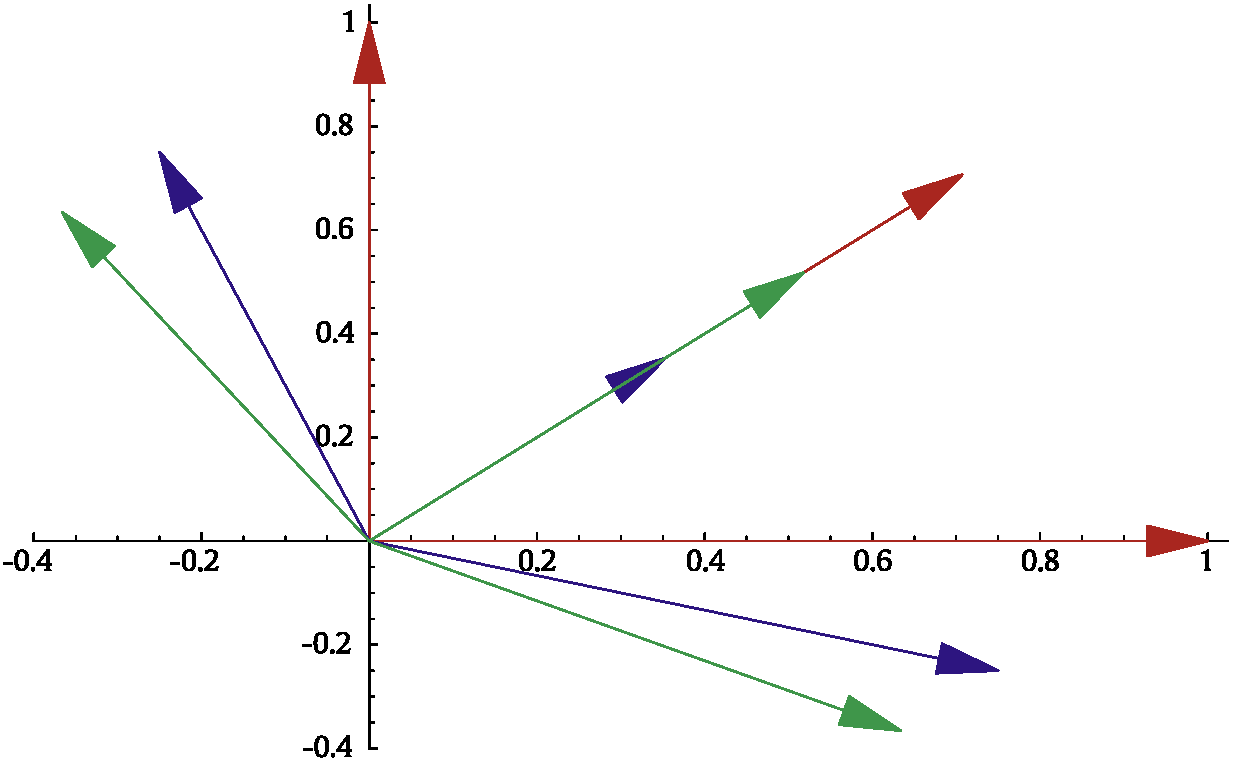
\includegraphics[scale=0.55]{image/frames.pdf}
  \caption{红色的为均匀长度的非Parseval框架,蓝色的为标准对偶框架,绿色的为最佳对偶框架.}
  \label{fig:3.1}
\end{figure}

\begin{proof}
最佳对偶框架是序列\(\{S^{-1}x_i+u_i\}_{i=1}^3\)满足极小极大问题
\[
	\min_{u_i}\max_{1\leqslant i\leqslant 3}\{\|S^{-1}x_i+u_i\|\},
\]
其中\(\sum_{i=1}^3\langle x,x_i\rangle u_i=0,\forall x\in\calH\),且典范对偶框架\(\{S^{-1}x_i\}_{i=1}^3\)为
\[
	\left\{\begin{bmatrix}
	3/4\\
	-1/4
	\end{bmatrix},
	\begin{bmatrix}
	-1/4\\
	3/4
	\end{bmatrix},
	\begin{bmatrix}
	1/2\sqrt{2}\\
	1/2\sqrt{2}
	\end{bmatrix}\right\}.
\]
置\(x_1=e_1,x_2=e_2\),则有
\begin{align*}
1u_1+0u_2+\frac{1}{\sqrt{2}}u_3&=0,\\
0u_1+1u_2+\frac{1}{\sqrt{2}}u_3&=0.
\end{align*}
因此满足条件的\(\{u_i\}_{i=1}^3\)具有如下的形式
\[
	u_1=u_2=\begin{bmatrix}
	a\\
	b
	\end{bmatrix},
	u_3=\begin{bmatrix}
	-\sqrt{2}a\\
	-\sqrt{2}b
	\end{bmatrix}.
\]
故需极小化的函数\(F(U)\)定义为
\[
	F(U)\coloneqq\max\big\{\|u+S^{-1}x_1\|,\|u+S^{-1}x_2\|,\|-\sqrt{2}u+S^{-1}x_3\|\big\},
\]
其中\(u=[a,b]^{\transpose}\).

为了简化计算,我们首先指出有最佳对偶框架满足\(a=b\). 这是可证的,若满足\(F(\tilde{u})\leqslant F(u)\),其中\(u=[a,b]^{\transpose},\tilde{u}=[(a+b)/2,(a+b)/2]^{\transpose}\).

设对合映射\(\dagger\)为
\begin{align*}
\dagger\colon\calH&\to\calH\\
                 u&\mapsto\hat{u}
\end{align*}                 
其中\(u=[a,b]^{\transpose},\hat{u}=[b,a]^{\transpose}\). 注意到\((S^{-1}x_1)^{\dagger}=S^{-1}x_2,(S^{-1}x_3)^{\dagger}=S^{-1}x_3\). 因此
\begin{align*}
F(\tilde{u})=&\max\Bigg\{\bigg\|\frac{u+u^{\dagger}}{2}+S^{-1}x_{1}\bigg\|,\bigg\|\frac{u+u^{\dagger}}{2}+S^{-1}x_{2}\bigg\|,\bigg\|\frac{-\sqrt{2}(u+u^{\dagger})}{2}+S^{-1}x_{3}\bigg\|\Bigg\}\\
=&\max\bigg\{\frac{1}{2}\big\|u+u^{\dagger}+2 S^{-1}x_{1}\big\|,\frac{1}{2}\big\|u+u^{\dagger}+2 S^{-1}x_{2}\big\|,\frac{\sqrt{2}}{2}\big\|u+u^{\dagger}-2/\sqrt{2}\cdot S^{-1}x_{3}\big\|\bigg\}\\
=&\max\bigg\{\frac{1}{2}\big\|(u+S^{-1} x_{1})+(u^{\dagger}+S^{-1}x_{1})\big\|,\frac{1}{2}\big\|(u+S^{-1}x_{2})+(u^{\dagger}+S^{-1}x_{2})\big\|,\\
&\frac{\sqrt{2}}{2}\big\|(u-1/\sqrt{2}\cdot S^{-1}x_{3})+(1/\sqrt{2}\cdot u^{\dagger}S^{-1}x_{3})\big\|\bigg\}\\
\leqslant&\max\bigg\{\frac{1}{2}\big(\big\|u+S^{-1} x_{1}\big\|+\big\|u^{\dagger}+S^{-1}x_{1}\big\|\big),\frac{1}{2}\big(\big\|u+S^{-1} x_{2}\big\|+\big\|u^{\dagger}+S^{-1}x_{2}\big\|\big),\\
&\frac{\sqrt{2}}{2}\big(\big\|u-1/\sqrt{2}\cdot S^{-1}x_{3}\big\|+\big\|u^{\dagger}-1/\sqrt{2}\cdot S^{-1}x_{3}\big\|\big)\bigg\}\\
=&\max\bigg\{\frac{1}{2}\big(\big\|u+S^{-1} x_{1}\big\|+\big\|\big(u+S^{-1}x_{2}\big)^{\dagger}\big\|\big),\frac{1}{2}\big(\big\|u+S^{-1}x_{2}\big\|+\big\|\big(u+S^{-1}x_{1}\big)^{\dagger}\big\|\big),\\
&\frac{\sqrt{2}}{2}\big(\big\|u-1/\sqrt{2}\cdot S^{-1}x_{3}\big\|+\big\|(u-1/\sqrt{2}\cdot S^{-1}x_{3}\big)^{\dagger}\big\|\big)\bigg\}\\
=&\max\bigg\{\frac{1}{2}\big(\|u+S^{-1} x_{1}\|+\|u+S^{-1}x_{2}\|\big),\frac{1}{2}\big(\|u+S^{-1}x_{2}\|+\|u+S^{-1}x_{1}\|\big),\\
&\sqrt{2}\big\|u-1/\sqrt{2}\cdot S^{-1}x_{3}\big\|\bigg\}\\
\leqslant&\max\big\{\big\|u+S^{-1} x_{1}\big\|,\big\|u+S^{-1} x_{2}\big\|,\big\|-\sqrt{2}u+S^{-1}x_{3}\big\|\big\}\\
=&F(u),
\end{align*}
其中最后一行是由不等式\((x+y)/2\leqslant\max(x,y),\forall x,y\geqslant 0\)得到的.

现置\(b=a\)且取范数的平方,我们希望寻求\(a\)使得\(f(a)\)极小
\[
	f(a)\coloneqq\max\{2a^2+a+5/8,2a^2+a+5/8,4a^2-2a+1/4\}.
\]

在\(a=(3-2\sqrt{2})/4\)时,\(f(a)\)是极小的,即
\[
	\min f(a)=\max\big\{(\sqrt{3}-1)^2,(\sqrt{3}-1)^2,(\sqrt{3}-1)^2\big\}=(\sqrt{3}-1)^2.
\]
因此
\[
	\left\{\begin{bmatrix}
	(3-\sqrt{3})/2\\[2pt]
	(1-\sqrt{3})/2
	\end{bmatrix},
	\begin{bmatrix}
	(1-\sqrt{3})/2\\[2pt]
	(3-\sqrt{3})/2
	\end{bmatrix},
	\begin{bmatrix}
	(\sqrt{3}-1)/\sqrt{2}\\[2pt]
	(\sqrt{3}-1)/\sqrt{2}
	\end{bmatrix}\right\}
\]
是\(\{x_i\}_{i=1}^3\)的一个最佳对偶框架. 事实上,置\(a=(3-2\sqrt{3})/4+r\),则\(f(a)\)的二次项变为
\[
	\begin{cases}
	(\sqrt{3}-1)^2+4r-2\sqrt{3}r+2r^2,\\
	(\sqrt{3}-1)^2+4r-4\sqrt{3}r+4r^2.
	\end{cases}
\]
为了使极大值小于\((\sqrt{3}-1)^2\),\(4r-2\sqrt{3}r+2r^2\)和\(4r-4\sqrt{3}r+4r^2\)需同时为负. 但\(4r-2\sqrt{3}r+2r^2\)仅在\(r=0\)或\(r=2-\sqrt{3}\)时为负,且\(4r-4\sqrt{3}r+4r^2\)仅在\(r=1-\sqrt{3}\)或\(r=0\)时为负,因此上述公式不可能同时为负. 故
\[
	\min\max\big\{2a^2+a+5/8,2a^2+a+5/8,4a^2-2a+1/4\big\}=(\sqrt{3}-1)^2.
\]

上述结论表明,在\(a=b\)时仅存在一个最佳对偶框架. 事实上,由于\(|\langle x,y\rangle|=\|x\|\|y\|\)当且仅当\(x\)与\(y\)线性无关,在\(a\ne b\)时易得
\begin{align*}
\big\|(u+S^{-1}x_1)+(u^{\dagger}+S^{-1}x_1)\big\|<&\text{ }\big\|u+S^{-1}x_1\big\|+\big\|u^{\dagger}+S^{-1}x_1\big\|,\\
\big\|(u+S^{-1}x_2)+(u^{\dagger}+S^{-1}x_2)\big\|<&\text{ }\big\|u+S^{-1}x_2\big\|+\|u^{\dagger}+S^{-1}x_2\big\|,\\
\big\|\big(u-1/\sqrt{2}\cdot S^{-1}x_3\big)+\big(u^{\dagger}-1/\sqrt{2}\cdot S^{-1}x_3\big)\big\|<&\text{ }\big\|u-1/\sqrt{2}\cdot S^{-1}x_3\big\|\\
&\text{ }+\big\|u^{\dagger}-1/\sqrt{2}\cdot S^{-1}x_3\big\|.
\end{align*}

因此在\(a\ne b\)的条件下,不等式\(F(\tilde{u})\leqslant F(u)\)是严格成立的. 故在\(a=b\)时最佳对偶框架存在且唯一.
\end{proof}

\begin{example}[具有无穷个最佳对偶框架的例子]
设\(\calH=\bbR^2\),考虑框架\(X=\{x_i\}_{i=1}^3\),即
\[
	\left\{\begin{bmatrix}
	1\\
	0
	\end{bmatrix},
	\frac{1}{2}\begin{bmatrix}
	0\\
	1
	\end{bmatrix},
	\frac{1}{2}\begin{bmatrix}
	0\\
	1
	\end{bmatrix}\right\}.
\]
此框架的框架算子及逆算子为
\[
	S=\begin{bmatrix}
	1&0\\
	0&1/2
	\end{bmatrix},
	\quad
	S^{-1}=\begin{bmatrix}
	1&0\\
	0&2
	\end{bmatrix},
\]
且标准对偶\(\{S^{-1}x_i\}_{i=1}^3\)为
\[
	\left\{\begin{bmatrix}
	1\\
	0
	\end{bmatrix},
	\begin{bmatrix}
	0\\
	1
	\end{bmatrix},
	\begin{bmatrix}
	0\\
	1
	\end{bmatrix}\right\}.
\]
故
\begin{align*}
\max_i\|S^{-1}x_i\|\cdot\|x_i\|&=\max\left\{
	1\cdot\left\|\begin{bmatrix}
	1\\
	0
	\end{bmatrix}\right\|,
	\frac{1}{2}\cdot\left\|\begin{bmatrix}
	0\\
	1
	\end{bmatrix}\right\|,
	\frac{1}{2}\cdot\left\|\begin{bmatrix}
	0\\
	1
	\end{bmatrix}\right\|\right\}\\
	&=\max\big\{1,1/2,1/2\big\}\\
	&=1.
\end{align*}
现考虑替代对偶框架\(\{S^{-1}x_i+h_i\}\),其中\(\{h_i\}_{i=1}^3\)为
\[
	\left\{\begin{bmatrix}
	0\\
	0
	\end{bmatrix},
	\begin{bmatrix}
	a\\
	b
	\end{bmatrix},
	\begin{bmatrix}
	-a\\
	-b
	\end{bmatrix}\right\},\quad\forall a,b\in\bbR.
\]
因此\(\|S^{-1}x_1+h_1\|\cdot\|x_1\|=\|S^{-1}x_1\|=1\)且选取\(a,b\)使得
\begin{align*}
\|S^{-1}x_2+h_2\|\cdot\|x_2\|&\leqslant 1,\\
\|S^{-1}x_3+h_3\|\cdot\|x_3\|&\leqslant 1,
\end{align*}
便给出了最佳对偶框架. 因此
\begin{align*}
\|S^{-1}x_2+h_2\|\cdot\|x_2\|&=\frac{1}{2}\cdot\left\|
\begin{bmatrix}
0\\
1
\end{bmatrix}+
\begin{bmatrix}
a\\
b
\end{bmatrix}\right\|\\
&=\frac{1}{2}\sqrt{a^2+(1+b)^2},\\
\|S^{-1}x_3+h_3\|\cdot\|x_3\|&=\frac{1}{2}\cdot\left\|
\begin{bmatrix}
0\\
1
\end{bmatrix}+
\begin{bmatrix}
-a\\
-b
\end{bmatrix}\right\|\\
&=\frac{1}{2}\sqrt{a^2+(1-b)^2}.
\end{align*}
因此对于任意的\(a,b\)满足条件
\[
	a^2+(1+b)^2\leqslant 4,\quad a^2+(1-b)^2\leqslant 4.
\]
由此可得到满足要求的\(a,b\)的取值区域,如图\ref{fig:3.2}所示.
\begin{figure}[h]
  \centering
  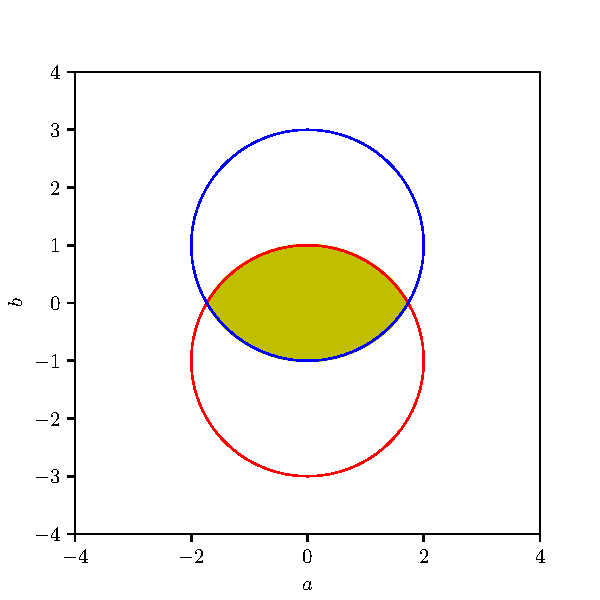
\includegraphics[scale=0.80]{image/ellipse_area.pdf}
  \caption{\(a,b\)取值区域示意图(图中黄色区域)}
  \label{fig:3.2}
\end{figure}

故在\(1\)丢失条件下有无穷多个最佳对偶框架.

最后,我们指出在\(2\)丢失的条件下此框架任具有无穷多个对偶框架. 设
\[
	V=\begin{bmatrix}
	1&0\\
	0&1/2\\
	0&1/2
	\end{bmatrix}
\]
并考虑\((V^{\dagger}+Z)DV,ZV=0\),且\(V^{\dagger}\)是最小平方逆.

则
\[
	Z=\begin{bmatrix}
	0&a&-a\\
	0&b&-b
	\end{bmatrix}.
\]
设\(E_{ij}\)是\(3\times 3\)的基本矩阵,即\((i,j)\)处的元素为\(1\)其余为\(0\)的矩阵. 则有
\begin{align*}
\calE_1=(V^{\dagger}+Z)E_{1,2}V&=\begin{bmatrix}
1&a/2\\
0&(1+b)/2
\end{bmatrix},\\
\calE_2=(V^{\dagger}+Z)E_{1,3}V&=\begin{bmatrix}
1&-a/2\\
0&(1-b)/2
\end{bmatrix},\\
\calE_3=(V^{\dagger}+Z)E_{2,3}V&=\begin{bmatrix}
0&0\\
0&1
\end{bmatrix}.
\end{align*}
范数是\(\calE\calE^{\star}\)最大特征值的平方根,且\(\|\calE_3\|=1\). 因此\(2\)丢失条件下的极大值是大于等于\(1\)的. 取\(a=b=0\),则\(\|\calE_1\|=\|\calE_2\|=1\).

由\(1\)丢失的最佳条件,我们已有
\begin{align*}
\frac{1}{2}\sqrt{a^2+(1+b)^2}&<1,\\[2pt]
\frac{1}{2}\sqrt{a^2+(1-b)^2}&<1.
\end{align*}

因此当\(a=0\)且\(b\)足够小时,则\(\|\calE_1\|=\|\calE_2\|=1\). 故在\(2\)丢失的条件下此框架有无穷多个对偶框架.
\end{example}

\newpage
\section*{致谢}
作者感谢审稿人提出的一些有益的建议,这些建议有助于改进本文的陈述方式.

\nocite{*}
\bibliography{wpref}

\end{document}
